\documentclass[10pt,a4paper]{article}
\usepackage{helvet}
\usepackage{graphicx} 
\usepackage{lastpage}
\usepackage{anysize}
\usepackage{fancyhdr}
\usepackage[german]{babel}
\usepackage[T1]{fontenc}
\usepackage[utf8]{inputenc}
\usepackage{aeguill}
\usepackage{eurosym}
\usepackage{multicol}

%%% Format der Seite anpassen
\marginsize{2.5cm}{2.5cm}{0.85cm}{4.11cm}
\renewcommand{\labelenumii}{\theenumi.\arabic{enumii}.}

%%% Header und Footer bauen
\pagestyle{fancy}
\renewcommand{\footrulewidth}{0.4pt}
\renewcommand{\headrulewidth}{0pt}
\renewcommand{\headheight}{2.75cm}
\renewcommand{\headsep}{0.5cm}
\setlength{\unitlength}{1mm}
\lhead{}
\lfoot{\small{(c) 2011-2014 by mars3142}}
\cfoot{\thepage\ / \pageref{LastPage}}
\rfoot{\small{Thx to Magellan}}

\begin{document}
\setlength{\parindent}{0mm}
\setlength{\parskip}{6pt }

%%% Dokumentenkrams nur auf der ersten Seite

\vspace{3.0cm}

\makebox[100.0mm][l]{\textbf{Titel}}
\makebox[20.0mm][l]{\textbf{Version}}
\makebox[37.0mm][r]{\textbf{Datum}} \\
\makebox[100.0mm][l]{Dokumentation WherUGo}
\makebox[20.5mm][l]{1.0}
\makebox[37.0mm][r]{\today}

\vspace{1cm}

%%% Dokumenteninhalt

\tableofcontents
\listoffigures

\section{Desktop}

\subsection{GWC-Viewer}
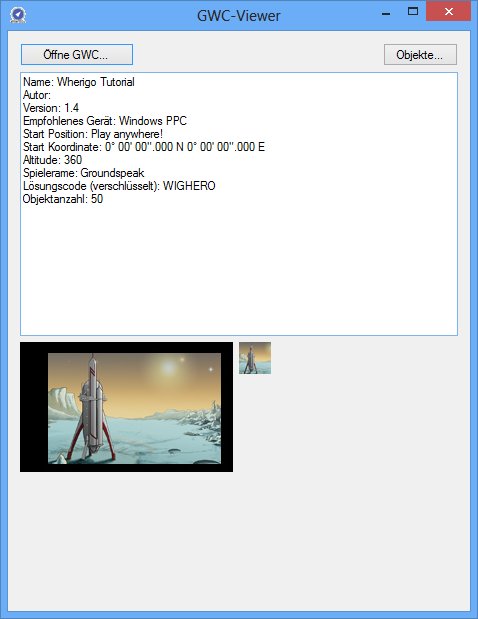
\includegraphics[width=0.5\textwidth]{screens/viewer_main}
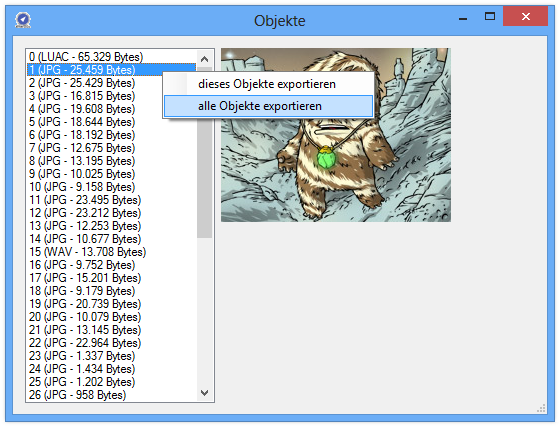
\includegraphics[width=0.5\textwidth]{screens/viewer_objects}

Der GWC-Viewer ist ein Hilfsmittel um zu sehen, welche Objekte (Sounds, Bilder) sich in dem Wherigo befinden. Diese kann man dann auch in den Ordner der Wherigo-Datei exportieren. Der LUA-Code (also das eigentliche Skript) ist compiliert und somit nicht lesbar, aber in einer sp"ateren Version des GWC-Viewers wird dieser Code auch dekompiliert sein.

\subsection{LuaTester}
Mit dem LuaTester wird es möglich sein, eigene Lua-Skripte auszuführen. Derzeit ist dieser noch nicht als Download verfügbar.

\section{Topic 2}
\subsection{Subtopic 1}
Proin luctus malesuada lectus id consequat. In felis lacus, sagittis non lobortis suscipit, sollicitudin et ante. Etiam nec metus metus. Nunc tincidunt facilisis magna, in vestibulum mauris rutrum ac. Nullam eget est in augue varius tempor. Cum sociis natoque penatibus et magnis dis parturient montes, nascetur ridiculus mus. Cras in ipsum lacus, semper sagittis massa. Donec dignissim venenatis venenatis. Curabitur ante tortor, sodales et tincidunt et, varius a nibh. Donec mollis sapien sit amet neque adipiscing placerat. Proin faucibus eros eget libero imperdiet sagittis.

\subsection{Subtopic 2}
Sed ornare ultrices venenatis. Sed eget tellus ante, non ornare eros. Vestibulum suscipit diam a libero commodo id volutpat neque cursus. Integer venenatis gravida libero sed consequat. Fusce egestas sagittis dui, quis tempor dolor euismod in. In hac habitasse platea dictumst. Fusce at ante leo. Ut felis sem, lacinia a vulputate luctus, iaculis non ipsum. Suspendisse potenti. Nullam vel erat nulla. Morbi at arcu ligula. Proin ultricies gravida sapien, in semper quam rutrum eget. Sed adipiscing condimentum sem id commodo. Aliquam vel odio quis risus molestie ultrices nec non neque. Vivamus sit amet metus vel sem mollis ultricies.

Proin luctus malesuada lectus id consequat. In felis lacus, sagittis non lobortis suscipit, sollicitudin et ante. Etiam nec metus metus. Nunc tincidunt         facilisis magna, in vestibulum mauris rutrum ac. Nullam eget est in augue varius tempor. Cum sociis natoque penatibus et magnis dis parturient montes, nascetur ridiculus mus. Cras in ipsum lacus, semper sagittis massa. Donec dignissim venenatis venenatis. Curabitur ante tortor, sodales et tincidunt et, varius a nibh.  Donec mollis sapien sit amet neque adipiscing placerat. Proin faucibus eros eget libero imperdiet sagittis.



\end{document}
